The libCEED \cite{libceed-user-manual} fluid dynamics mini-application solves the time-dependent Navier-Stokes equations of compressible gas dynamics in a static Eulerian three-dimensional frame using unstructured high-order finite element spatial discretizations and explicit or implicit high-order time-stepping.
Moreover, since the Navier-Stokes example has been developed using PETSc, the pointwise physics represented in the quadrature point function ${\color{applegreen}\mathbf{D}}$ are separated from the parallelization, meshing, and linear and non-linear solvers.

The mathematical formulation used in the fluid dynamics mini-application is similar to the discussion in \cite{giraldoetal2010}.
The compressible Navier-Stokes equations in conservative form are given by
\begin{equation}
   \begin{aligned}
   \frac{\partial \rho}{\partial t} + \nabla \cdot \mathbf{U} &= 0 \\
   \frac{\partial \mathbf{U}}{\partial t} + \nabla \cdot \left( \frac{\mathbf{U} \otimes \mathbf{U}}{\rho} + P \mathbf{I}_3 - \mathbf\sigma \right) + \rho g \hat{\mathbf{k}} &= 0 \\
   \frac{\partial E}{\partial t} + \nabla \cdot \left( \frac{(E + P)\mathbf{U}}{\rho} -\mathbf{u} \cdot \mathbf{\sigma} - k \nabla T \right) &= 0 \, , \\
   \end{aligned}
\label{eq:ns}
\end{equation}
where $\boldsymbol{\sigma} = \mu \left( \nabla \mathbf{u} + \left( \nabla \mathbf{u} \right)^T + \lambda \left( \nabla \cdot \mathbf{u} \right) \mathbf{I}_3 \right)$ is the Cauchy (symmetric) stress tensor, with $\mu$ the dynamic viscosity coefficient, and $\lambda = - 2/3$ the Stokes hypothesis constant.
In Equation \ref{eq:ns}, $\rho$ represents the volume mass density, $\mathbf{U}$ the momentum density (defined as $\mathbf{U} = \rho \mathbf{u}$, where $\mathbf{u}$ is the vector velocity field), $E$ the total energy density (defined as $E = \rho e$, where $e$ is the total energy), $\mathbf{I}_3$ represents the $3 \times 3$ identity matrix, $g$ the gravitational acceleration constant, $\mathbf{\hat{k}}$ the unit vector in the $z$ direction, $k$ the thermal conductivity constant, $T$ represents the temperature, and $P$ the pressure.
Pressure is given by the equation of state
\begin{equation}
   P = \left( {c_p}/{c_v} -1\right) \left( E - {\mathbf{U} \cdot \mathbf{U}}/{(2 \rho)} - \rho g z \right) \, ,
   \label{eq:ns_state}
\end{equation}
where $c_p$ is the specific heat at constant pressure and $c_v$ is the specific heat at constant volume (that define $\gamma = c_p / c_v$, the specific heat ratio).

The system in Equation \ref{eq:ns} can be rewritten in vector form
\begin{equation}
   \frac{\partial \mathbf{q}}{\partial t} + \nabla \cdot \mathbf{F}(\mathbf{q}) -S(\mathbf{q}) = 0 \, ,
\label{eq:vector-ns}
\end{equation}
for the state variables 5-dimensional vector
\begin{equation}
    \mathbf{q} =
           \begin{pmatrix}
               \rho \\
               \mathbf{U} \equiv \rho \mathbf{u}\\
               E \equiv \rho e
           \end{pmatrix}
           \begin{array}{l}
               \leftarrow\textrm{ volume mass density}\\
               \leftarrow\textrm{ momentum density}\\
               \leftarrow\textrm{ energy density}
           \end{array}
\end{equation}
where the flux and the source terms, respectively, are given by
\begin{equation}
    \begin{aligned}
    \mathbf{F}(\mathbf{q}) &=
    \begin{pmatrix}
        \mathbf{U}\\
        {(\mathbf{U} \otimes \mathbf{U})}/{\rho} + P \mathbf{I}_3 -  \boldsymbol{\sigma} \\
        {(E + P)\mathbf{U}}/{\rho} - \mathbf{u}  \cdot \boldsymbol{\sigma} - k \nabla T
    \end{pmatrix} ,\\
    S(\mathbf{q}) &=
    - \begin{pmatrix}
        0\\
        \rho g \mathbf{\hat{k}}\\
        0
    \end{pmatrix}.
    \end{aligned}
\end{equation}

Let the discrete solution be
\begin{equation}
   \mathbf{q}_N (\mathbf{x},t)^{(e)} = \sum_{k = 1}^{p + 1}\phi_k (\mathbf{x})\mathbf{q}_k^{(e)}
\end{equation}
with $p + 1$ being the number of nodes on the element $e$ and $\phi$ represents the finite elment basis functions.

For the time discretization, we use two types of time-stepping schemes, explicit and implicit.

\subsubsection{Explicit Time-Stepping Formulation}

The explicit formulation for the adaptive Runge-Kutta-Fehlberg (RKF4-5) method is given by
\begin{equation}
       \mathbf{q}_N^{n+1} = \mathbf{q}_N^n + \Delta t \sum_{i=1}^{s} b_i k_i \, ,
\end{equation}
where
\begin{equation}
       \begin{aligned}
          k_1 &= f(t^n, \mathbf{q}_N^n)\\
          k_2 &= f(t^n + c_2 \Delta t, \mathbf{q}_N^n + \Delta t (a_{21} k_1))\\
          k_3 &= f(t^n + c_3 \Delta t, \mathbf{q}_N^n + \Delta t (a_{31} k_1 + a_{32} k_2))\\
          \vdots&\\
          k_i &= f\left(t^n + c_i \Delta t, \mathbf{q}_N^n + \Delta t \sum_{j=1}^s a_{ij} k_j \right)\\
       \end{aligned}
\end{equation}
and with
\begin{equation}
       f(t^n, \mathbf{q}_N^n) = - [\nabla \cdot \mathbf{F}(\mathbf{q}_N)]^n + [S(\mathbf{q}_N)]^n \, .
\end{equation}
Note that any explicit time-stepping scheme available in PETSc can be chosen at runtime.

\subsubsection{Implicit Time-Stepping Formulation}

The implicit formulation solves nonlinear systems for $\mathbf q_N$, given by
\begin{equation}
       \mathbf f(\mathbf q_N) \equiv \mathbf g(t^{n+1}, \mathbf{q}_N, \mathbf{\dot{q}}_N) = 0 \, ,
       \label{eq:ts-implicit-ns}
\end{equation}
where the time derivative $\mathbf{\dot q}_N$ is defined by
\begin{equation}
      \mathbf{\dot{q}}_N(\mathbf q_N) = \alpha \mathbf q_N + \mathbf z_N
\end{equation}
in terms of $\mathbf z_N$ from prior state and $\alpha > 0$, both of which depend on the specific time integration scheme.

To determine how difficult a given non-linear time integration problem is to solve, consider the Jacobian of Equation \ref{eq:ts-implicit-ns},
\begin{equation}
       \frac{\partial \mathbf f}{\partial \mathbf q_N}
       = \frac{\partial \mathbf g}{\partial \mathbf q_N}
       + \alpha \frac{\partial \mathbf g}{\partial \mathbf{\dot q}_N}.
\end{equation}

The scalar shift $\alpha$ scales inversely with the time step $\Delta t$, so small time steps result in the Jacobian being dominated by the second term, which is a sort of "mass matrix", and typically well-conditioned independent of grid resolution with a simple preconditioner.
In contrast, the first term dominates for large time steps, with a condition number that grows with the diameter of the domain and polynomial degree of the approximation space.
Both terms are significant for time-accurate simulation and the setup costs of strong preconditioners must be balanced with the convergence rate of Krylov methods using weak preconditioners.

To obtain a finite element discretization, we first multiply the strong form in Equation \ref{eq:vector-ns} by a test function $\mathbf v \in H^1 \left( \Omega \right)$ and integrate,
\begin{equation}
   \int_{\Omega} \mathbf v \cdot \left(\frac{\partial \mathbf{q}_N}{\partial t} + \nabla \cdot \mathbf{F}(\mathbf{q}_N) - \mathbf{S}(\mathbf{q}_N) \right) \,dV = 0 \, , \; \forall \mathbf v \in \mathcal{V}_p\,,
\end{equation}
with $\mathcal{V}_q = \{ \mathbf v(\mathbf x) \in H^{1} \left( \Omega_e \right) \,|\, \mathbf v(\mathbf x_e(\mathbf X)) \in P_q(\mathbf{I}), e = 1,\ldots,N_e \}$ a mapped space of polynomials containing at least polynomials of degree $q$, with or without the higher mixed terms that appear in tensor product spaces.

Integrating by parts on the divergence term, we arrive at the weak form,
\begin{equation}
   \begin{aligned}
   \int_{\Omega} \mathbf v \cdot \left( \frac{\partial \mathbf{q}_N}{\partial t} - \mathbf{S}(\mathbf{q}_N) \right)  \,dV
   - \int_{\Omega} \nabla \mathbf v \!:\! \mathbf{F}(\mathbf{q}_N)\,dV & \\
   + \int_{\partial \Omega} \mathbf v \cdot \mathbf{F}(\mathbf q_N) \cdot \hat{\mathbf{n}} \,dS
     &= 0 \, , \; \forall \mathbf v \in \mathcal{V}_p \,,
   \end{aligned}
   \label{eq:weak-vector-ns}
\end{equation}
where $\mathbf{F}(\mathbf q_N) \cdot \hat{\mathbf{n}}$ is typically replaced with a boundary condition.

\begin{figure}[ht!]
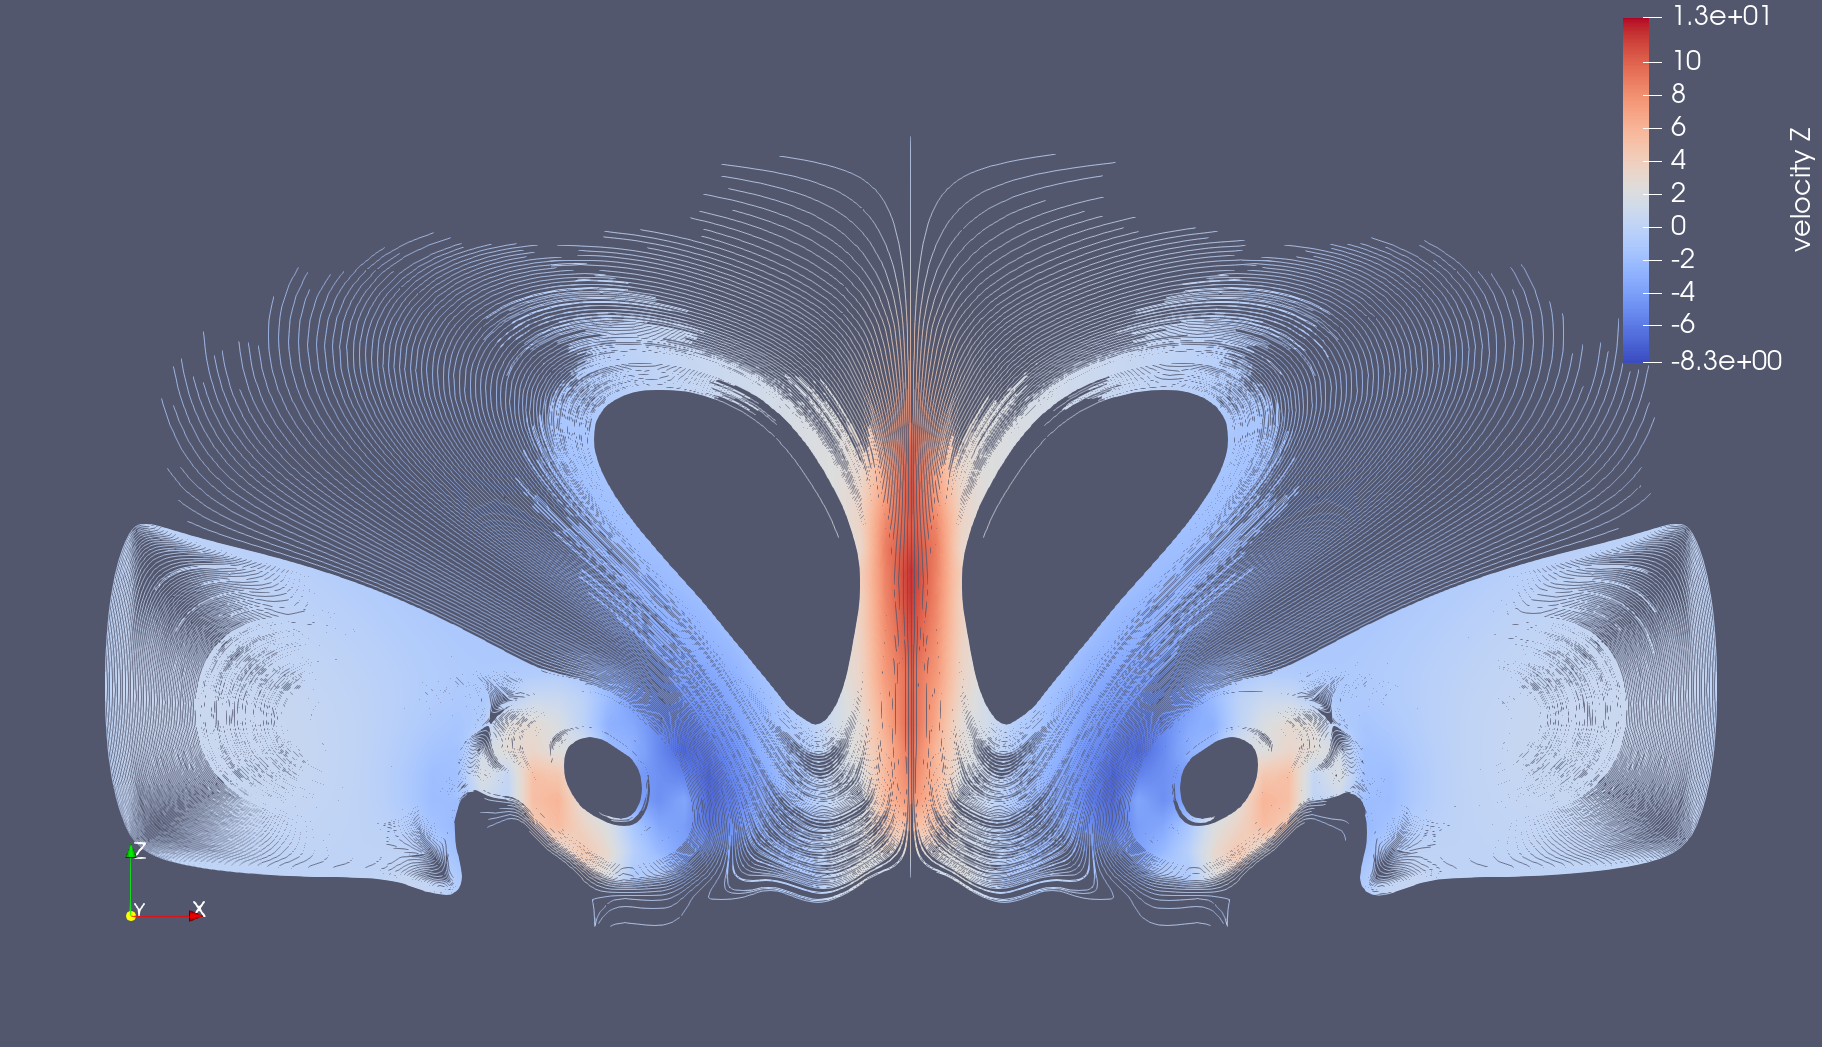
\includegraphics[width=.99\linewidth]{../img/Vortices}
\caption{Vortices Developing as a Cold Air Bubble Drops to the Ground}
\label{fig:vortices}
\end{figure}

Figure \ref{fig:vortices} shows an atmospheric simulation where vortices develop as a cold air bubble drops to the ground.
This mini-application can run on host or device processors and supports stabilization techniques such as streamline-upwind (SU) and streamline-upwind Petrov-Galerkin (SUPG).
